% Payload-Aware Two-Tier UAV Route Planning — Review I Presentation

\documentclass[aspectratio=169,11pt]{beamer}

% ---------- Theme and colours ----------
\usetheme{Madrid}
\usecolortheme{default}
\definecolor{UniversityBlue}{RGB}{16,62,110}
\definecolor{AccentBlue}{RGB}{30,136,229}
\definecolor{LightBlue}{RGB}{232,242,252}
\definecolor{DarkGray}{RGB}{55,65,81}

\setbeamercolor{structure}{fg=UniversityBlue}
\setbeamercolor{palette primary}{bg=UniversityBlue,fg=white}
\setbeamercolor{palette secondary}{bg=AccentBlue,fg=white}
\setbeamercolor{frametitle}{bg=UniversityBlue,fg=white}
\setbeamercolor{block title}{bg=UniversityBlue,fg=white}
\setbeamercolor{block body}{bg=LightBlue,fg=black}
\setbeamercolor{alerted text}{fg=AccentBlue}

% ---------- Packages ----------
\usepackage[T1]{fontenc}
\usepackage[utf8]{inputenc}
\usepackage{lmodern}
\usepackage{graphicx}
\graphicspath{{../diagrams/}{./}}
\usepackage{booktabs}
\usepackage{array}
\usepackage{tabularx}
\usepackage{tikz}
\usetikzlibrary{positioning}
\usepackage{amsmath}
\usepackage{listings}
\usepackage{xcolor}
\usepackage{colortbl}
\usepackage{microtype}
\usepackage{hyperref}

\newcolumntype{Y}{>{\raggedright\arraybackslash}X}

% ---------- General settings ----------
\setbeamertemplate{navigation symbols}{}
\setbeamertemplate{caption}[numbered]
\setbeamertemplate{itemize item}{\color{AccentBlue}$\blacktriangleright$}
\setbeamertemplate{itemize subitem}{\color{UniversityBlue}$\bullet$}
\setbeamersize{text margin left=0.7cm,text margin right=0.7cm}

% Footer: project title, institution and slide number
\setbeamertemplate{footline}{%
  \leavevmode%
  \hbox{%
    \begin{beamercolorbox}[wd=.42\paperwidth,ht=2.7ex,dp=1.1ex,leftskip=.6em]{author in head/foot}%
      \insertshorttitle
    \end{beamercolorbox}%
    \begin{beamercolorbox}[wd=.46\paperwidth,ht=2.7ex,dp=1.1ex,center]{date in head/foot}%
      Department of Computer Science and Engineering
    \end{beamercolorbox}%
    \begin{beamercolorbox}[wd=.12\paperwidth,ht=2.7ex,dp=1.1ex,center]{page number in head/foot}%
      \insertframenumber/\inserttotalframenumber
    \end{beamercolorbox}%
  }%
  \vskip0pt%
}

% ---------- Editable project details ----------
\title[Payload-Aware Two-Tier UAV Route Planning]{%
  Payload-Aware Two-Tier UAV Route Planning\\for Last-Mile Delivery}
\subtitle{Review Report -- I}
\author[Thirumurugan $\cdot$ Meghna $\cdot$ Shrika]{%
  \texorpdfstring{%
    \begin{tabular}{l@{\hspace{1.5cm}}r}
      Thirumurugan RA & (3122235001149) \\
      Meghna Manimaran & (3122235001079) \\
      Shrika SP Thota & (3122235001125)
    \end{tabular}%
  }{Thirumurugan RA, Meghna Manimaran, Shrika SP Thota}%
}
\institute[SSN College of Engineering]{%
  Guided by: Sujaudeen N, Assistant Professor\\[2mm]
  Department of Computer Science and Engineering\\
  Sri Sivasubramaniya Nadar College of Engineering%
}
\date{Academic Year 2026--2027}
\hypersetup{
  pdftitle={Payload-Aware Two-Tier UAV Route Planning for Last-Mile Delivery},
  pdfauthor={Thirumurugan RA, Meghna Manimaran, Shrika SP Thota}
}

\begin{document}

% ── 1. Title slide ──────────────────────────────────────────────────────────
\begin{frame}[plain]
  \titlepage
\end{frame}

% ── 2. Outline ──────────────────────────────────────────────────────────────
\begin{frame}{Presentation Outline}
  \tableofcontents
\end{frame}

% ════════════════════════════════════════════════════════════════
\section{Introduction}
% ════════════════════════════════════════════════════════════════

% ── 3. Background and Motivation ────────────────────────────────────────────
\begin{frame}{Background and Motivation}
  \begin{columns}[T,onlytextwidth]
    \column{0.58\textwidth}
      \begin{itemize}
        \item UAVs are an effective platform for last-mile delivery where ground transport is impractical: remote clinics, emergency drug drops, and fragile diagnostic sample transport.
        \item Every flight must balance three \textbf{conflicting objectives}: total distance, battery energy use, and exposure to high-risk flight segments.
        \item Existing routing systems treat all deliveries \textbf{identically} — a fragile medical device and a robust parcel travel the \emph{same} route.
        \item Payload metadata (fragility, urgency, payload weight) encodes routing priorities, but \textbf{no system exploits this at mission time}.
      \end{itemize}
    \column{0.38\textwidth}
      \begin{block}{Core Motivation}
        Payload-blind UAV routing pipelines cannot adapt to cargo-specific constraints.  A two-tier architecture that bridges payload semantics directly to Pareto route selection addresses this structural gap.
      \end{block}
  \end{columns}
\end{frame}

% ── 3b. Real-World Evidence (NEW) ───────────────────────────────────────────
\begin{frame}{Real-World Cost of Payload-Blind Routing}
  \begin{block}{Swiss Post -- Matternet M2 Crashes (Z\"{u}rich, Jan \& May 2019)~\cite{r12}}
    \footnotesize Drones carrying clinical laboratory specimens flew \textbf{fixed, payload-invariant
    routes}. Post-incident analysis confirmed identical corridors regardless of cargo type ---
    no routing adjustment for payload fragility.
  \end{block}
  \vspace{0.05cm}
  \begin{block}{Vibration \& Turbulence Degradation Studies~\cite{r13,r14,r15}}
    \footnotesize Controlled lab work shows drone-transported medicines degrade measurably:
    insulin fibrillation, biologic protein denaturation, elevated haemolysis in blood samples
    on high-vibration segments.  Altitude variation and turbulence raise lab rejection rates.
  \end{block}
  \vspace{0.05cm}
  \begin{block}{Zipline Rwanda Blood-Delivery Network (up to 80\,km/charge)~\cite{r16}}
    \footnotesize Heavier blood-product payloads draw more hover/lift power and shorten range,
    yet the system flies the same fixed route regardless of payload weight ---
    no energy-efficient detour for heavy cargo, no direct short route for urgent light payload.
  \end{block}
  \vspace{0.04cm}
  \centering\footnotesize\textbf{Root cause in every case:} the planner does not know what is
  carried, so it cannot prefer smoother corridors for fragile payloads or shortest paths for
  time-critical medicine.
\end{frame}

% ── 4. Problem Statement ────────────────────────────────────────────────────
\begin{frame}{Problem Statement}
  \begin{alertblock}{Problem}
    Existing UAV routing systems apply \textbf{static, cargo-agnostic
    objective weights}, resulting in \textbf{suboptimal or unsafe routes}
    for payloads with differing fragility, urgency, and payload weight.
  \end{alertblock}
  \vspace{0.05cm}
  \begin{itemize}
    \item Given payload metadata $(F,\,W,\,U,\,P_\mathrm{lvl})$ with
          $F\in\{1\ldots5\}$, $W\in\{1\ldots3\}$, $U\in\{1\ldots3\}$,
          $P_\mathrm{lvl}\in\{1\ldots5\}$, and airspace graph $G=(V,E)$,
          select route $p^*$ from the Pareto front that best satisfies
          payload requirements --- no expert re-tuning, no re-running the search.
    \item Single-objective routing collapses all objectives into one scalar and
          cannot model their three-way conflict.
    \item No existing system maps payload description to Pareto point selection
          via an explicit algebraic formula.
    \item Constraints: selection must be deterministic, reproducible, and finish
          within 1\,s of payload tag entry.
  \end{itemize}
\end{frame}

% ── 4b. Response to Review 0 Panel (NEW) ────────────────────────────────────
\begin{frame}{Review 0: Feedback \& Actions}
  \scriptsize
  \begin{tabularx}{\textwidth}{>{\bfseries\raggedright\arraybackslash}p{3.6cm} Y}
    \toprule
    \textbf{Panel Comment} & \textbf{Resolution in Current Work}\\
    \midrule
    ``No correlation between Tier~1 and Tier~2 factors'' &
      Explicit algebraic mapping introduced: Fragility $F$ scales
      $w_\mathrm{risk}$; Urgency $U$ scales $w_\mathrm{dist}$; Payload
      weight $W$ scales $w_\mathrm{energy}$.  Every Tier~2 tag maps to a
      Tier~1 objective via a closed formula.\\[5pt]
    ``Criteria are not considered to map together'' &
      The formula $w_\mathrm{risk}=(F{\times}2)\,/\,(F{\times}2+U{\times}3+W{\times}2)$
      (and equivalents) is a continuous function --- all four tags simultaneously
      influence all three weights; changing any single tag shifts all three weights
      proportionally.\\[5pt]
    ``Application of Pareto needs rethinking'' &
      Extreme-point selection \textbf{replaced} by utility scoring over the
      \emph{full} Pareto front:
      $\mathrm{score}(p_i)=w_d(1{-}\tilde{d}_i)+w_\varepsilon(1{-}\tilde{\varepsilon}_i)+w_\rho(1{-}\tilde{\rho}_i)$.
      Mixed-priority payloads select \emph{non-extreme interior points} that
      no single-objective baseline can produce.\\[5pt]
    ``Complexity only in Tier~2; more than 2 objectives'' &
      Tier~1 manages three-objective NAMOA* graph-search complexity;
      Tier~2 manages metadata-to-weight mapping and full-front utility scoring.
      Both tiers carry distinct computational roles --- neither reduces to a
      single-objective problem.\\
    \bottomrule
  \end{tabularx}
\end{frame}

% ── 5. Objectives ───────────────────────────────────────────────────────────
\begin{frame}{Project Objectives}
  \begin{enumerate}
    \item To build a \textbf{multi-objective A* engine (Tier~1)} that
          constructs a Pareto-optimal route set over an airspace graph,
          balancing distance, energy consumption, and flight risk simultaneously.
    \item To design an \textbf{algebraic bridge} that translates payload
          metadata tags (fragility~$F$, payload weight~$W$, urgency~$U$,
          priority~$P_\mathrm{lvl}$) into normalised routing objective
          weights with no expert tuning.
    \item To implement a \textbf{Tier~2 payload-driven selector} that scores
          every Pareto route using the derived weights and returns the
          utility-maximising route~$p^*$.
    \item To evaluate the pipeline using \textbf{simulation benchmarks} on
          50, 200, and 500-node graphs against single-objective A* and MOPSO
          baselines, using hypervolume, Pareto spread, IGD, and Tier~2
          selection accuracy.
    \item To validate the system on \textbf{real drone hardware}
          (Raspberry Pi~5 + Pixhawk) through ArduPilot SITL simulation and
          outdoor flight tests.
  \end{enumerate}
\end{frame}

% ── 6. Scope ────────────────────────────────────────────────────────────────
\begin{frame}{Scope and Expected Outcomes}
  \begin{columns}[T,onlytextwidth]
    \column{0.48\textwidth}
      \begin{block}{Included}
        \begin{itemize}
          \item Payload-aware UAV route selection for single-drone delivery
          \item Two-tier pipeline: Pareto front construction + utility-based
                Pareto point selection
          \item Software simulation on OSM graphs
                (Thiruvanmiyur, Chennai)
          \item ArduPilot SITL + RPi~5 + Pixhawk hardware integration and
                outdoor flight tests
          \item Benchmark against single-objective A* and MOPSO
        \end{itemize}
      \end{block}
    \column{0.48\textwidth}
      \begin{block}{Excluded / Constraints}
        \begin{itemize}
          \item Multi-UAV fleet management and coordination
          \item Real-time dynamic obstacle avoidance during flight
          \item Commercial deployment and regulatory compliance
          \item Weather-based in-flight re-routing
          \item Deep-learning-based risk estimation
        \end{itemize}
      \end{block}
  \end{columns}
\end{frame}

% ════════════════════════════════════════════════════════════════
\section{Literature Review}
% ════════════════════════════════════════════════════════════════

% ── 7. Literature table (UPDATED) ───────────────────────────────────────────
\begin{frame}{Literature Review}
  \scriptsize
  \begin{tabularx}{\textwidth}{%
      >{\raggedright\arraybackslash}p{2.6cm}
      >{\raggedright\arraybackslash}p{3.0cm}
      >{\raggedright\arraybackslash}p{2.8cm}
      >{\raggedright\arraybackslash}X}
    \toprule
    \textbf{Author / Year} & \textbf{Method} &
    \textbf{Key Contribution} & \textbf{Limitation / Research Gap}\\
    \midrule
    Chokkalingam \& Ganesan (2026)~\cite{r1} &
      Pareto-entropy PSO (POPSO) with dynamic parameter adaptation &
      Entropy-guided archiving improves front diversity; adaptable to
      real-time environmental changes &
      Final route still a manually re-tuned weighted sum per mission;
      payload metadata never incorporated --- fragile samples and
      emergency medicine get the same hand-tuned selection\\
    \addlinespace
    Tsoutsouras et al.\ (2020)~\cite{r10} &
      Mass-aware flight-speed and energy-model adaptation for
      multi-drop trajectories &
      Reduces energy consumption vs.\ mass-agnostic planning across
      multi-stop routes &
      Continuous mass used only inside the energy/speed model itself;
      builds no multi-objective Pareto front; discrete payload metadata
      (fragility, urgency) plays no role in route selection\\
    \addlinespace
    Ren et al.\ (2019)~\cite{r3} &
      Crowding-distance NSGA-II (CDNSGA-II) over octree urban
      environment &
      Well-spread, collision-free Pareto-optimal paths in urban
      airspace &
      Crowding distance encodes only geometric front spread; urgency,
      fragility, and payload weight play no role in selection\\
    \bottomrule
  \end{tabularx}
\end{frame}

% ── 8. Gap and novelty (UPDATED — Gap 1/2/3) ────────────────────────────────
\begin{frame}{Research Gap and Proposed Contribution}
  \begin{columns}[T,onlytextwidth]
    \column{0.47\textwidth}
      \begin{block}{Three Identified Gaps}
        \begin{itemize}
          \item \textbf{Gap~1:} No payload-aware route \emph{selection} ---
                all planners apply a fixed geometric criterion independent of
                payload type, or no selection mechanism at all
          \item \textbf{Gap~2:} No front reuse --- full multi-objective
                search re-run whenever mission context changes
          \item \textbf{Gap~3:} No algebraic bridge --- no formalised
                mapping from payload description to the routing trade-off it
                implies
        \end{itemize}
      \end{block}
    \column{0.49\textwidth}
      \begin{block}{Proposed Contribution (closes all three)}
        \begin{itemize}
          \item Tier~2 maps four payload tags directly to Pareto point
                selection via formula \textbf{(Gap~1)}
          \item Front refreshed periodically; Tier~2 selects per mission
                against current front --- no re-run \textbf{(Gap~2)}
          \item Closed-form bridge:
                $F,W,U \!\rightarrow\! w_\mathrm{risk},w_\mathrm{dist},w_\mathrm{energy}$
                \textbf{(Gap~3)}
          \item $p^* = \arg\max_{p_i\in\mathcal{P}}\operatorname{score}(p_i)$
                --- selects non-extreme interior points for mixed payloads
        \end{itemize}
      \end{block}
  \end{columns}
\end{frame}

% ════════════════════════════════════════════════════════════════
\section{System Design}
% ════════════════════════════════════════════════════════════════

% ── 9. Existing vs Proposed (UPDATED variable names T→W) ────────────────────
\begin{frame}{Existing System vs.\ Proposed System}
  \small
  \begin{tabularx}{\textwidth}{>{\bfseries\raggedright\arraybackslash}p{2.9cm}YY}
    \toprule
    Criterion & Existing Routing Systems & Proposed Two-Tier System\\
    \midrule
    Routing approach &
      Single-objective (distance or energy only) &
      Multi-objective NAMOA* --- distance, energy, and risk simultaneously\\
    Payload handling &
      Cargo-agnostic; all parcels treated identically &
      Payload tags $(F,W,U,P_\mathrm{lvl})$ derive objective weights
      algebraically\\
    Route selection &
      Single greedy path or extreme Pareto point; expert re-tunes weights
      per mission &
      Utility scoring over full Pareto front; selects non-extreme interior
      points for mixed payloads\\
    Front reuse &
      Full search re-run on every mission context change &
      Front built once per region; Tier~2 selects in $<$1\,s against
      current front\\
    Hardware validation &
      Simulation only &
      ArduPilot SITL + RPi~5 + Pixhawk outdoor flight tests\\
    \bottomrule
  \end{tabularx}
\end{frame}

% ── 10a. Methodology ─────────────────────────────────────────
\begin{frame}{Proposed Methodology}
  \centering
  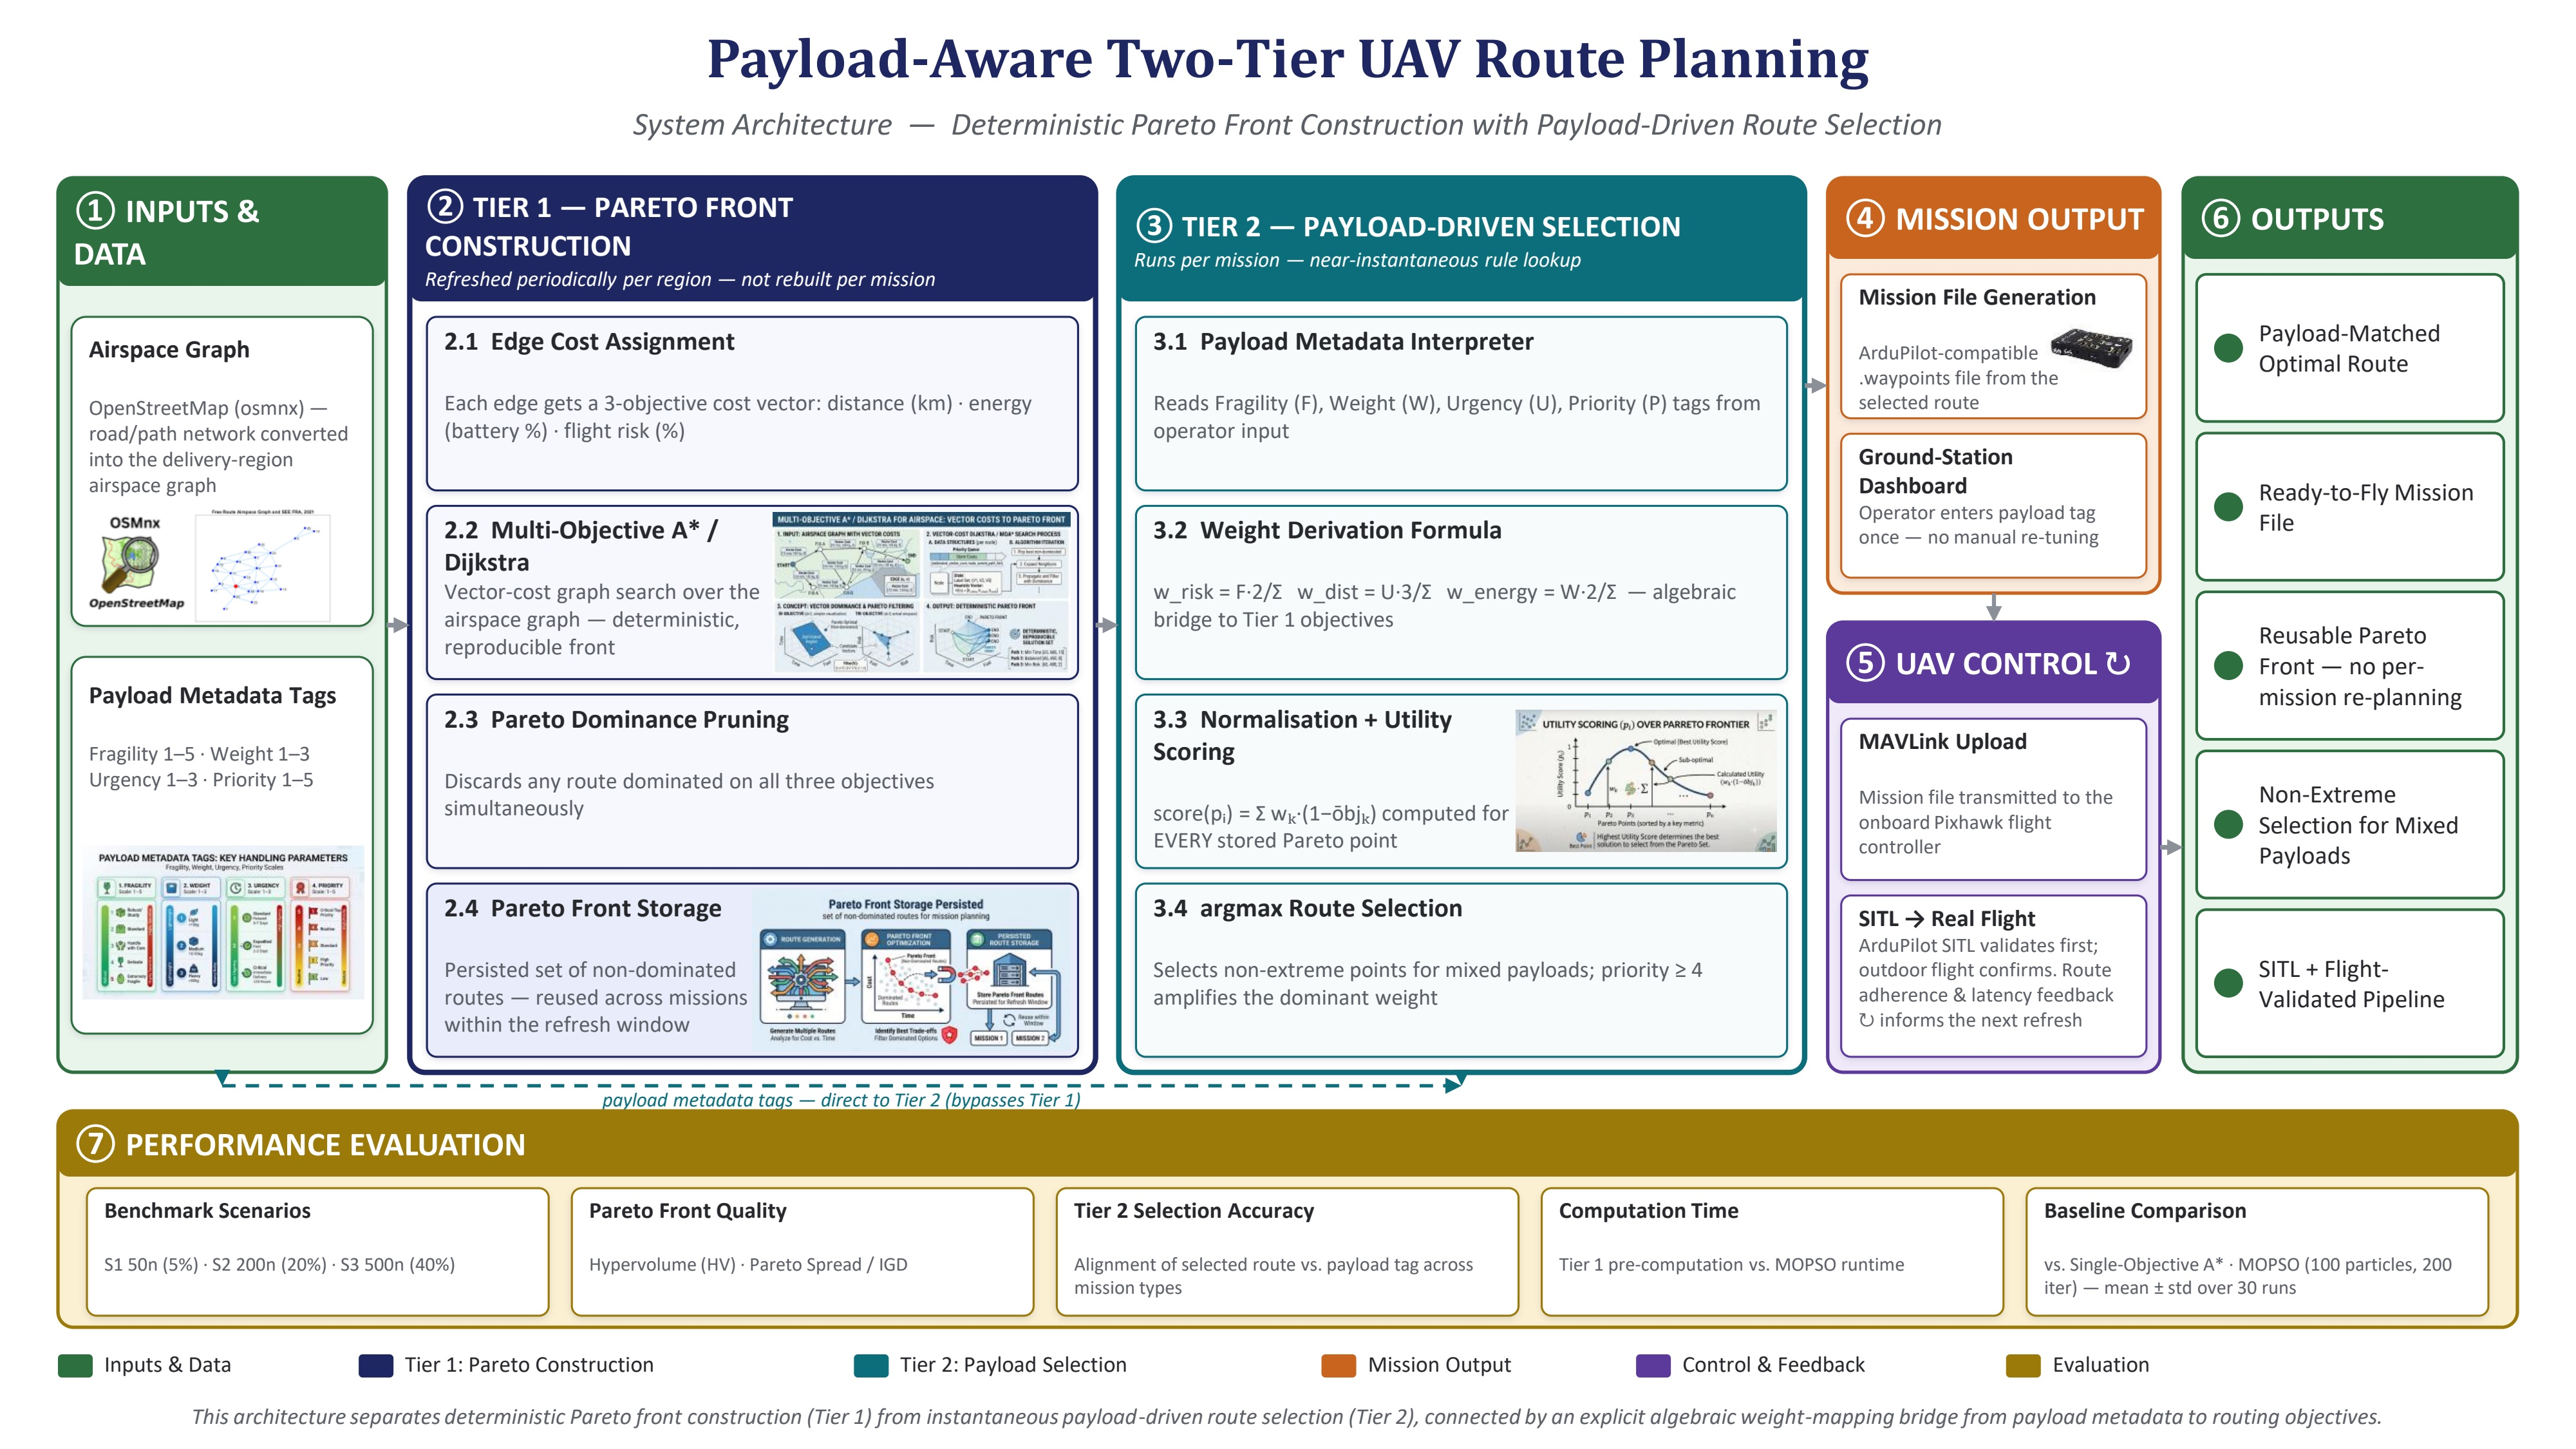
\includegraphics[width=1\textwidth,height=0.95\textheight,
                   keepaspectratio]{Methodology Diagram.jpg}

  \vspace{0.15cm}
\end{frame}

% ── 10b. Architecture ────────────────────────────────────────────────────────
\begin{frame}{Proposed System Architecture}
  \centering
  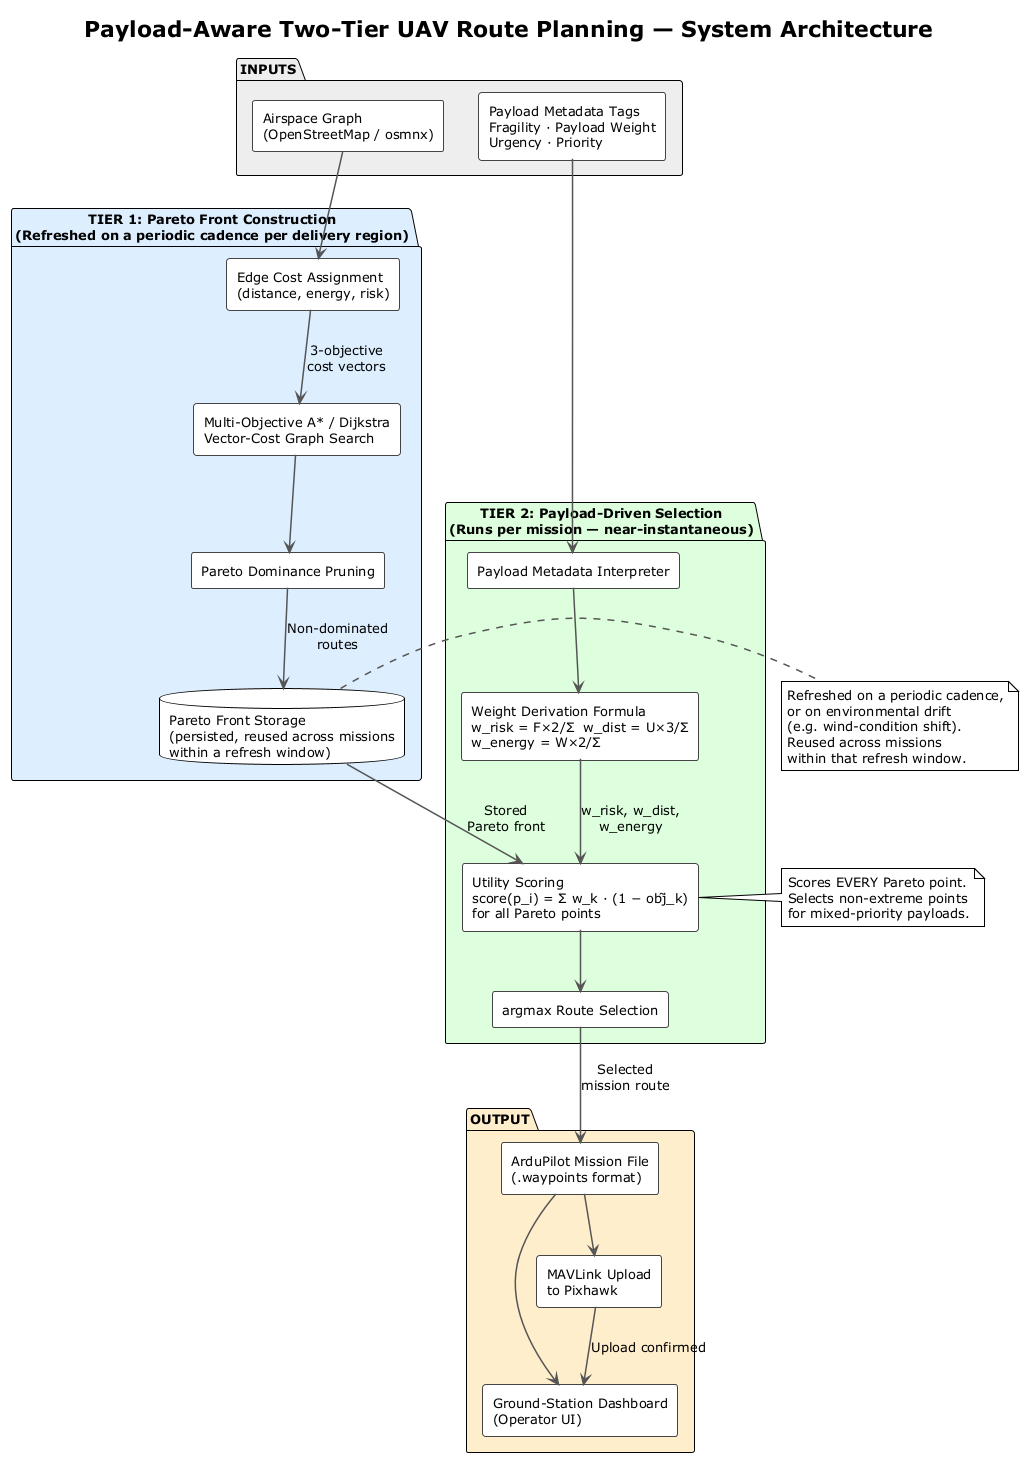
\includegraphics[width=1\textwidth,height=0.85\textheight,keepaspectratio]{arch.png}
\end{frame}

% ── 11. Modules ─────────────────────────────────────────────────────────────
\begin{frame}{System Modules}
  \begin{enumerate}
    \item \textbf{M1 -- Airspace Graph Builder:}
          Extracts OSM road/path network via \texttt{osmnx}; assigns three
          objective costs to each edge: geodesic distance, energy
          (distance $\times$ altitude-change factor), and flight risk
          (simulated threat zones and obstacle density, scored 0--1).

    \item \textbf{M2 -- Multi-Objective A* Engine (Tier~1):}
          NAMOA* search maintaining a cost vector $\mathbf{g}=[d,\varepsilon,\rho]$
          per partial path; node-level label-dominance pruning; stores
          deterministic Pareto front $\mathcal{P}$ on disk for Tier~2 reuse.

    \item \textbf{M3 -- Payload Metadata Interpreter (Tier~2):}
          Reads tags $(F,W,U,P_\mathrm{lvl})$; derives $w_\mathrm{risk},
          w_\mathrm{dist},w_\mathrm{energy}$ via closed formula; min-max
          normalises objectives; returns $\arg\max$ route and generates
          ArduPilot \texttt{.waypoints} mission file.

    \item \textbf{M4 -- Testing and Evaluation:}
          Benchmarks on S1/S2/S3 graphs vs.\ single-objective A* and MOPSO
          (30 runs); metrics: hypervolume, Pareto spread ($\Delta$), IGD,
          Tier~2 selection accuracy, computation time.  Extends to ArduPilot
          SITL and outdoor flight tests.
  \end{enumerate}
\end{frame}

% ── 12. Methodology ─────────────────────────────────────────────────────────
\begin{frame}{Methodology / Workflow}
  \begin{columns}[T,onlytextwidth]
    \column{0.62\textwidth}
      \begin{enumerate}
        \item Literature review and problem formulation
        \item Airspace graph construction (OpenStreetMap + OSMnx)
        \item Multi-objective A* (NAMOA*) engine implementation (Tier~1)
        \item Algebraic bridge and payload-driven Pareto selector (Tier~2)
        \item Software simulation and benchmarking vs.\ A* and MOPSO baselines
        \item Hardware integration (RPi~5 + Pixhawk), ArduPilot SITL
              simulation, and outdoor flight validation
      \end{enumerate}
    \column{0.34\textwidth}
      \begin{block}{Evaluation Metrics}
        \begin{itemize}
          \item Hypervolume (HV)
          \item Pareto spread ($\Delta$ metric)
          \item IGD vs.\ reference front
          \item Tier~2 selection accuracy
          \item Tier~1 computation time
          \item Route adherence (GPS error)
        \end{itemize}
      \end{block}
  \end{columns}
\end{frame}

% ── 13. Algorithm ─────────────────
\begin{frame}{Core Algorithm: Payload-Aware Two-Tier Route Planning}
  \begin{block}{Algorithm Summary}
    \begin{enumerate}
      \item \textbf{Input:} Graph $G=(V,E)$, payload tags
            $(F,W,U,P_\mathrm{lvl})$, source $s$, destination $d$.
      \item \textbf{Weight derivation (Algebraic Bridge):}\\
            $r_\mathrm{raw}{=}F{\times}2$,\quad
            $d_\mathrm{raw}{=}U{\times}3$,\quad
            $e_\mathrm{raw}{=}W{\times}2$;\quad
            normalise $\Rightarrow w_\mathrm{risk},\,w_\mathrm{dist},\,w_\mathrm{energy}$.\\
            If $P_\mathrm{lvl}\geq4$: amplify dominant weight by
            $0.1{\times}w_\mathrm{max}$, then renormalise to sum to 1.
      \item \textbf{Tier~1 (NAMOA*):} Run multi-objective A*;
            maintain cost vectors; apply node-level label-dominance pruning;
            store Pareto front $\mathcal{P}$ on disk for reuse.
      \item \textbf{Tier~2 --- Utility Scoring:} For each $p_i\in\mathcal{P}$,
            \[
              \operatorname{score}(p_i)=
                w_\mathrm{dist}(1-\tilde{d}_i)
                +w_\mathrm{energy}(1-\tilde{\varepsilon}_i)
                +w_\mathrm{risk}(1-\tilde{\rho}_i)
            \]
      \item \textbf{Output:}
            $p^*=\arg\max_{p_i\in\mathcal{P}}\operatorname{score}(p_i)$;
            generate ArduPilot \texttt{.waypoints} file; upload via MAVLink.
    \end{enumerate}
  \end{block}
\end{frame}

% ── 14. Activity Flow Diagrams ──────────────────────────────────────────────────
\begin{frame}{Activity Flow Diagrams for Two-Tier Architecture}
  \begin{columns}[T,onlytextwidth]
    \column{0.48\textwidth}
      \centering
      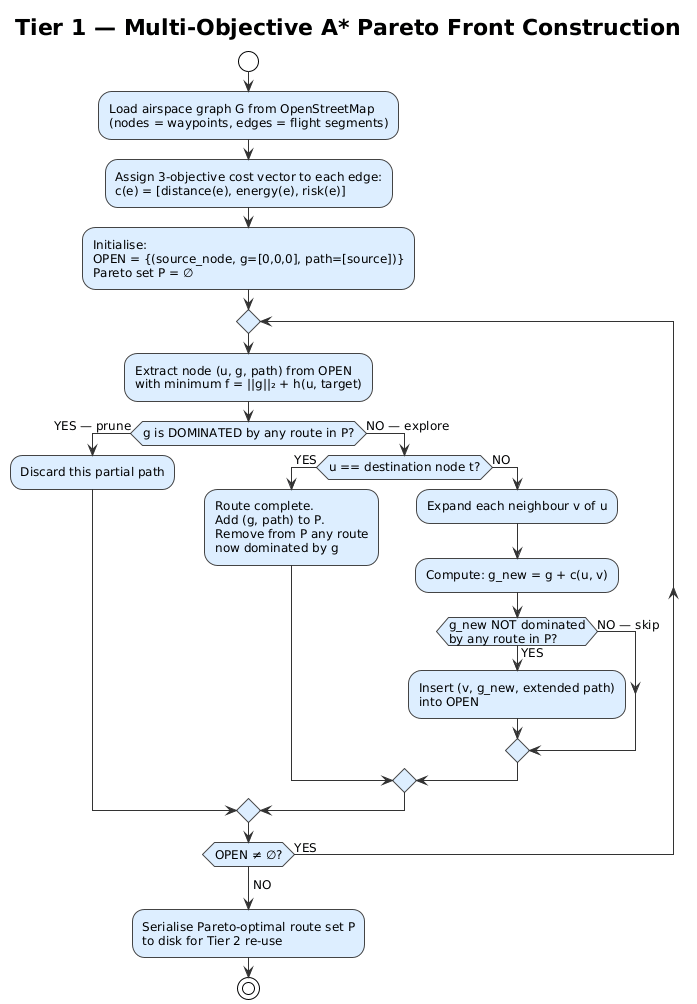
\includegraphics[width=\linewidth,height=6.35cm,keepaspectratio]{tier1.png}

      \small Tier~1: Multi-Objective A* (NAMOA*) Pareto Front Construction
    \column{0.48\textwidth}
      \centering
      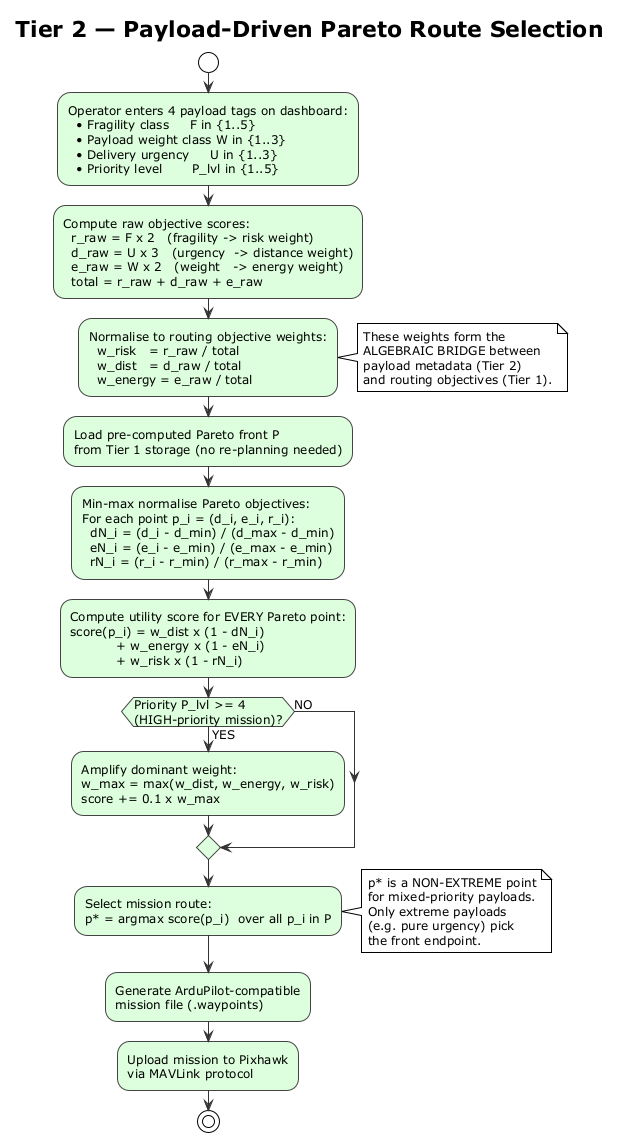
\includegraphics[width=\linewidth,height=6.35cm,keepaspectratio]{tier2.png}

      \small Tier~2: Payload-Driven Pareto Route Selection
  \end{columns}
\end{frame}

% ── 15. Technology stack ────────────────────────────────────────────────────
\begin{frame}{Technology Stack and Resources}
  \small
  \begin{tabularx}{\textwidth}{>{\bfseries\raggedright\arraybackslash}p{3.2cm}Y}
    \toprule
    Category & Selected Technology / Resource\\
    \midrule
    Programming language  & Python 3.11\\
    Core libraries        & NetworkX, OSMnx, NumPy, matplotlib, SciPy\\
    Communication protocol & MAVLink / ArduPilot \texttt{.waypoints}
                             mission format\\
    Simulation environment & ArduPilot SITL (primary validation before
                             real flights)\\
    Map / dataset          & OpenStreetMap airspace graph
                             (Thiruvanmiyur, Chennai urban area)\\
    Development tools      & Git, VS Code, QGIS, Mission Planner,
                             ArduPilot SITL, Docker\\
    Hardware               & Raspberry Pi~5 (quad-core 2.4\,GHz, 8\,GB),
                             Pixhawk~6C, GPS module, F450 frame,
                             ESC + motors\\
    \bottomrule
  \end{tabularx}
\end{frame}

% ════════════════════════════════════════════════════════════════
\section{Implementation and Results}
% ════════════════════════════════════════════════════════════════

% ── 16. Implementation status (Phase I — software scope) ───
\begin{frame}{Implementation Status}
  \scriptsize
  \renewcommand{\arraystretch}{1.0}
  \begin{tabularx}{\textwidth}{Y>{\centering\arraybackslash}p{2.3cm}Y}
    \toprule
    \textbf{Component} & \textbf{Status} & \textbf{Evidence / Remarks}\\
    \midrule
    Literature review \& problem formulation &
      Completed &
      3 papers surveyed; 3 gaps formalised; real-world evidence added\\
    System design \& architecture &
      Completed &
      Two-tier architecture, NAMOA* algorithm, and algebraic bridge
      designed; diagrams produced\\
    Airspace graph construction &
      In Progress &
      Actively building the airspace graph model and 3-objective edge-cost
      assignment for the target delivery region\\
    Tier~1: Multi-Objective A* (NAMOA*) engine &
      Planned &
      NAMOA* with 3-objective cost vectors + label-dominance pruning
      specified; implementation scheduled for Phase~II\\
    Tier~2: Payload-driven selector &
      Planned &
      Algebraic bridge and utility-scoring $\arg\max$ selection formalised;
      coding scheduled for Phase~II\\
    Benchmarking \& evaluation &
      Planned &
      Metrics defined (HV, $\Delta$, IGD, selection accuracy, runtime);
      benchmark harness vs.\ single-obj.\ A* and MOPSO planned for Phase~II\\
    \bottomrule
  \end{tabularx}
\end{frame}

% ── 17. Results ─────────────────────────────────────────────────────────────
\begin{frame}{Expected Results and Performance Targets}
  \begin{columns}[T,onlytextwidth]
    \column{0.54\textwidth}
      \begin{block}{Payload Preset Weight Derivation}
        \scriptsize
        \begin{tabularx}{\linewidth}{Y c c c}
          \toprule
          \textbf{Preset} &
          $w_\mathrm{risk}$ & $w_\mathrm{dist}$ & $w_\mathrm{energy}$\\
          \midrule
          Fragile medical ($F{=}5,W{=}1,U{=}1$)
            & 0.667 & 0.200 & 0.133\\
          Emergency medicine ($F{=}1,W{=}1,U{=}3$)
            & 0.144 & 0.712 & 0.144\\
          Disaster relief ($F{=}1,W{=}3,U{=}1$)
            & 0.182 & 0.273 & 0.545\\
          Mixed cargo ($F{=}3,W{=}2,U{=}2$)
            & 0.375 & 0.375 & 0.250\\
          \bottomrule
        \end{tabularx}
        \vspace{0.04cm}
        Only emergency medicine selects an extreme Pareto point.
        \textbf{All other presets select non-extreme interior points} no
        single-objective baseline can produce.
      \end{block}
    \column{0.42\textwidth}
      \begin{block}{Performance Targets}
        \begin{itemize}
          \item HV: $\geq$20\% higher than single-obj.\ A*
          \item Pareto front: 5--20 non-dominated routes per scenario
          \item Tier~2 selection latency: $<$50\,ms on RPi~5
          \item Tier~2 accuracy: correct priority objective ranked highest
                across all 4 presets
          \item Hardware: ArduPilot SITL + outdoor delivery flight
        \end{itemize}
      \end{block}
  \end{columns}
  \vspace*{-3pt}
\end{frame}

% ── 18. Testing ─────────────────────────────────────────────────────────────
\begin{frame}{Testing and Validation Plan}
  \scriptsize
  \begin{tabularx}{\textwidth}{p{1.2cm} Y Y p{2.0cm}}
    \toprule
    \textbf{Test ID} & \textbf{Test Scenario} &
    \textbf{Expected Result} & \textbf{Status}\\
    \midrule
    TC-01 & Valid payload tags $(F,W,U,P_\mathrm{lvl})$ input &
      Correct $w_\mathrm{risk},w_\mathrm{dist},w_\mathrm{energy}$ derived;
      weights sum to 1.0 &
      Planned\\
    TC-02 & NAMOA* on 50/200/500-node graphs (S1/S2/S3) &
      Pareto front with zero dominated routes; HV $>$ single-obj.\ A* &
      Planned\\
    TC-03 & High fragility ($F{=}5$) vs.\ emergency medicine ($U{=}3$) &
      Significantly different non-extreme routes selected from same front &
      Planned\\
    TC-04 & Disconnected graph (no feasible path) &
      Graceful error with clear user message &
      Planned\\
    TC-05 & RPi~5 MAVLink mission upload to Pixhawk via SITL &
      Drone accepts mission and executes flight in ArduPilot SITL &
      Planned\\
    \bottomrule
  \end{tabularx}
  \vspace{0.25cm}
  \begin{block}{Validation Method}
    Unit tests (pytest), MOPSO benchmarking (30 runs, swarm\,=\,100,
    200 iterations), ArduPilot SITL integration tests, and outdoor UAV
    flight tests with GPS telemetry logs.
  \end{block}
\end{frame}

% ════════════════════════════════════════════════════════════════
\section{Project Management}
% ════════════════════════════════════════════════════════════════

% ── 19. Timeline ────────────────────────────────────────────────────────────
\begin{frame}{Project Timeline (Jul\,2026 -- Mar\,2027)}
  \scriptsize
  \begin{tabularx}{\textwidth}{Y*{9}{>{\centering\arraybackslash}p{0.56cm}}}
    \toprule
    \textbf{Activity} &
    \textbf{Jul} & \textbf{Aug} & \textbf{Sep} & \textbf{Oct} &
    \textbf{Nov} & \textbf{Dec} & \textbf{Jan} & \textbf{Feb} &
    \textbf{Mar}\\
    \midrule
    Literature survey \& formulation &
      \cellcolor{AccentBlue!35} & \cellcolor{AccentBlue!35} &
      \cellcolor{AccentBlue!35} &&&&&&\\
    System design \& architecture &
      & \cellcolor{AccentBlue!35} & \cellcolor{AccentBlue!35} &&&&&& \\
    Tier~1: Multi-Objective A* &&&
      \cellcolor{AccentBlue!35} & \cellcolor{AccentBlue!35} &&&&&\\
    Tier~2: Payload-Driven Selector &&&&
      \cellcolor{AccentBlue!35} & \cellcolor{AccentBlue!35} &&&&\\
    Software simulation \& benchmarking &&&&&
      \cellcolor{AccentBlue!35} & \cellcolor{AccentBlue!35} &&&\\
    Hardware integration (RPi~5 + Pixhawk) &&&&&&
      \cellcolor{AccentBlue!35} & \cellcolor{AccentBlue!35} &&\\
    Outdoor flight tests &&&&&&&
      \cellcolor{AccentBlue!35} & \cellcolor{AccentBlue!35} &\\
    Documentation \& report writing &&&&&&&
      & \cellcolor{AccentBlue!35} & \cellcolor{AccentBlue!35}\\
    \bottomrule
  \end{tabularx}
  \vspace{0.2cm}
  \small
  \textcolor{UniversityBlue}{\textbf{Review I:}} August 2026\qquad
  \textcolor{UniversityBlue}{\textbf{Final Submission:}} March 2027
\end{frame}

% ── 20. Responsibilities (ALL In Progress) ──────────────────────────────────
\begin{frame}{Team Responsibilities}
  \small
  \begin{tabularx}{\textwidth}{>{\bfseries\raggedright\arraybackslash}p{3.3cm}Y p{2.3cm}}
    \toprule
    Team Member & Responsibilities & Current Status\\
    \midrule
    Thirumurugan RA &
      System architecture design, Tier~1 NAMOA* engine implementation,
      airspace graph construction (OSMnx), edge cost vectorization &
      In Progress\\
    Meghna Manimaran &
      Algebraic bridge design, Tier~2 payload selector implementation,
      benchmarking suite development, documentation &
      In Progress\\
    Shrika SP Thota &
      Literature survey \& problem formulation, risk-cost model design,
      benchmarking methodology, Pareto-front visualization and result analysis &
      In Progress\\
    \bottomrule
  \end{tabularx}
\end{frame}

% ════════════════════════════════════════════════════════════════
\section{Conclusion}
% ════════════════════════════════════════════════════════════════

% ── 21. Challenges ──────────────────────────────────────────────────────────
\begin{frame}{Challenges, Risks, and Mitigation}
  \small
  \begin{tabularx}{\textwidth}{Y Y Y}
    \toprule
    \textbf{Risk / Challenge} & \textbf{Possible Impact} &
    \textbf{Mitigation}\\
    \midrule
    Graph complexity (large OSM urban network) &
      Slow Pareto front construction &
      Spatial pruning, NAMOA* node-level label-dominance check,
      epsilon-dominance to limit front size\\
    Hardware failure (RPi / Pixhawk) &
      Flight tests delayed &
      ArduPilot SITL validation first; spare hardware budget\\
    Pareto front size too large &
      High memory and selection latency &
      Apply epsilon-pruning; front bounded to $\leq$100 routes\\
    MAVLink integration issues &
      Mission upload failures &
      Validate protocol end-to-end in SITL before real drone flights\\
    \bottomrule
  \end{tabularx}
\end{frame}

% ── 22. Conclusion and Future Work ──────────────────────────────────────────
\begin{frame}{Conclusion and Future Work}
  \begin{block}{Conclusion}
    This project addresses the critical gap of payload-blind UAV routing by
    proposing a two-tier payload-aware pipeline.  Tier~1 builds a Pareto-optimal
    route set via NAMOA*; Tier~2 selects the mission route using an algebraic
    bridge that maps fragility, urgency, and payload weight to routing
    objective weights.  Utility scoring over the full Pareto front replaces
    context-blind diversity criteria, enabling non-extreme route selection for
    mixed payloads that no single-objective baseline can produce.
  \end{block}
  \begin{block}{Future Work}
    \begin{itemize}
      \item Outdoor flight validation on a real RPi~5 + Pixhawk drone in a
            simulated urban delivery environment.
      \item Extend to multi-drone coordination with shared Pareto fronts.
      \item Incorporate real-time weather and dynamic obstacle data for
            in-flight re-routing with adaptive front refresh thresholds.
    \end{itemize}
  \end{block}
\end{frame}

% ── 23. References ────────────────────────────────────────────────
\begin{frame}[allowframebreaks]{References}
  \footnotesize
  \begin{thebibliography}{99}

    \bibitem{r1}
      B.\ Chokkalingam and V.\ Ganesan,
      ``Pareto-optimal particle swarm optimisation with entropy-based
      archive selection for UAV path planning,''
      \emph{RAIRO -- Operations Research}, 2026.
      DOI: 10.1051/ro/2025159

    \bibitem{r3}
      Y.\ Ren et al.,
      ``Crowding-distance-based NSGA-II for multi-objective UAV path
      planning in urban environments,''
      in \emph{Proc.\ IEEE SOSE}, 2019.
      DOI: 10.1109/SOSE.2019.00059

    \bibitem{r4}
      G.\ Boeing,
      ``OSMnx: New methods for acquiring, constructing, analysing, and
      visualising complex street networks,''
      \emph{Computers, Environment and Urban Systems}, vol.~65,
      pp.~126--139, 2017.
      DOI: 10.1016/j.compenvurbsys.2017.05.004

    \bibitem{r5}
      A.\ Hagberg, P.\ Swart, and D.\ Chult,
      ``Exploring network structure, dynamics, and function using
      NetworkX,'' in \emph{Proc.\ 7th Python in Science Conf.\ (SciPy)},
      pp.~11--15, 2008.

    \bibitem{r6}
      C.\ A.\ C.\ Coello, G.\ T.\ Pulido, and M.\ S.\ Lechuga,
      ``Handling multiple objectives with particle swarm optimization,''
      \emph{IEEE Trans.\ Evolutionary Computation}, vol.~8, no.~3,
      pp.~256--279, 2004.
      DOI: 10.1109/TEVC.2004.826067

    \bibitem{r7}
      L.\ Meier et al.,
      ``MAVLink: Micro air vehicle communication protocol,'' 2013.
      [Online]. Available: \url{https://mavlink.io}

    \bibitem{r10}
      V.\ Tsoutsouras et al.,
      ``Multi-objective trajectory optimisation for energy-efficient UAV
      delivery with payload-mass adaptation,''
      arXiv:2001.02531 [eess.SY], 2020.

    \bibitem{r12}
      Swiss Federal Office of Civil Aviation (FOCA),
      Post-incident analysis of Swiss Post -- Matternet M2 drone crashes,
      Z\"{u}rich, January and May 2019.

    \bibitem{r13}
      R.\ Rosser et al.,
      ``Effect of unmanned aerial vehicle transport on the stability of
      insulin: a controlled study,''
      \emph{Diabetes Care}, 2019.

    \bibitem{r14}
      R.\ Amukele et al.,
      ``Drone transport of chemistry and hematology samples over long
      distances,''
      \emph{Am.\ J.\ Clin.\ Pathol.}, 2017.

    \bibitem{r15}
      D.\ Bhatt et al.,
      ``Hemolysis in blood samples transported by drone: a comparative
      study,''
      \emph{Clin.\ Biochem.}, 2021.

    \bibitem{r16}
      B.\ Tapper et al.,
      ``Energy analysis of long-range blood-product delivery by fixed-wing
      UAV: lessons from Zipline Rwanda,''
      \emph{J.\ Unmanned Veh.\ Syst.}, 2022.

  \end{thebibliography}
\end{frame}

% ── 24. Thank You ───────────────────────────────────────────────────────────
\begin{frame}[plain]
  \centering
  \vfill
  {\usebeamerfont{title}\color{UniversityBlue}\Huge Thank You}\par
  \vspace{0.5cm}
  {\Large Questions and Discussion}\par
  \vspace{0.8cm}
  {\normalsize
    Thirumurugan RA\quad$\cdot$\quad
    Meghna Manimaran\quad$\cdot$\quad
    Shrika SP Thota}\par
  \vspace{0.3cm}
  {\small Guide: Sujaudeen N, Assistant Professor}
  \vfill
\end{frame}

\end{document}
